{A water tank has the shape of an truncated, inverted pyramid, with dimensions given below, and is filled with water with a mass density of 1000 kg/m$^3$. Find the work performed in pumping all water to a point 1 m above the top of the tank.

\hfill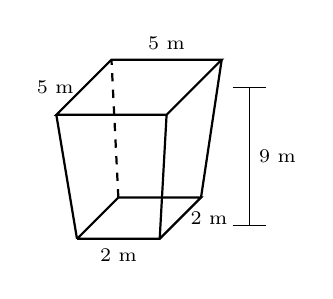
\begin{tikzpicture}[xscale=.7,yscale=.7]
\draw [thick] (0,0) node (A) {}-- node [pos=.5,left]{\scriptsize 5 m} (1,1)node (B) {} --node [above,pos=.5] {\scriptsize 5 m} (3,1) node (C) {} -- (2,0) node (D) {}--cycle;
\begin{scope}[scale=.75,shift={(.5,-3)}]
\draw [thick] (0,0) node (AA) {} -- (1,1) node (BB) {} -- (3,1) node (CC) {} -- node [right,pos=.5] {\scriptsize 2 m} (2,0) node (DD) {}-- node [pos=.5,below]{\scriptsize 2 m} (0,0);
\end{scope}
\draw [dashed,thick] (BB.center) -- (B.center);
\draw [thick] (AA.center) -- (A.center)
							(DD.center) -- (D.center)
							(CC.center) -- (C.center);
\draw (3.2,.5) -- (3.8,.5)
			(3.2,-2) -- (3.8,-2)
			(3.5,.5) -- node [pos=.5,right] {\scriptsize 9 m} (3.5,-2);\end{tikzpicture}
\hfill\null
}
{4,917,150 J
}
